% !TeX root = ../main.tex
% !TeX spelling = en_GB
% !TeX program = pdflatex

\chapter{Materials, Methods and Unpublished Results}
\label{chap:methods}

The work begun with some initial tests, in which different light sources and illumination angles were investigated. It was decided to use a shadowgraph system with background illumination. The experimental setup was tested using different water droplet generators and a test target consisting of micrometer sized lines and dots. Analyzing the optical system and testing different segmentation algorithms we found a simple way to define the sample volume from a single image. Using the Laplacian of Gaussian edge detection, which principally is a second derivation of the image intensity gradient, and a suitable threshold, we can create closed curves around objects where the edge is in or near focus. To test the ability of measuring concentration we needed to build a weather protected prototype that could be used in parallell with a second instrument. The prototype needed to be fully automatic, able to analyze images in real time 24 hours a day during several months and store the results in a compressed format. To calibrate the size measurement and the measurement range, the previously mentioned dots of different sizes were used. The size measurement was also verified using distributions polymer microspheres, applied by blowing compressed air through a glass dispenser.

\section{Image Segmentation}

Detection can be done in several ways. The simplest method is to use a threshold at a fixed level and define the edge as the transition between above and below that threshold \cite{gonz2002}. This technique is Other techniques use different methods to measure the gradient of the change in intensity \cite{canny1986,marr1980}.

\section{Optical Characteristica}

As simplificaiton we describe the measured droplets as spherical lenses made of pure water at a constant temperature, surrounded by air. 

\subsection{Light Spectrum}

Although water is a good absorber of electromagnetic ratiation in most spectral wavelenghts except for the visible, the volume of water droplets is too small for the absorbtion to be measurable. In visible light, the water droplet can be regarded as a spherical lens with a very short focal length, thus spreading most of the light in diverging directions. Since the used camera is specifically designed for visible and near infrared, we tested and compared two different wavelenghts, 455 nm and 850 nm using the same optical setup. The shorter wavelength gave sharper images.

\begin{figure}
\centering
\begin{minipage}{.5\textwidth}
  \centering
  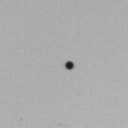
\includegraphics[width=.6\linewidth]{figures/compare455nmdot}
  %\caption{A subfigure}
  %\label{fig:compare455nmdot}
\end{minipage}%
\begin{minipage}{.5\textwidth}
  \centering
  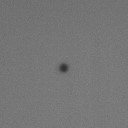
\includegraphics[width=.6\linewidth]{figures/compare850nmdot}
  %\caption{A subfigure}
  %\label{fig:compare850nmdot}
\end{minipage}
\caption{Same dot viewed in different background light. 455 nm (left) and 850 nm (right).}
\label{fig:comparedots}
\end{figure}

One would expect diffraction patterns depending on the spectral bandwith of the light source. The narrower band width the stronger the diffraction would be. A spectrum analyze of the LED showed that the coherence length of the blue LED is about 6.8 μm. Therefore the spectrum was measured using a spectrum analyzer. The result can be seen in Figure \ref{fig:ledspectrum}

\begin{figure}%[ht]
\centering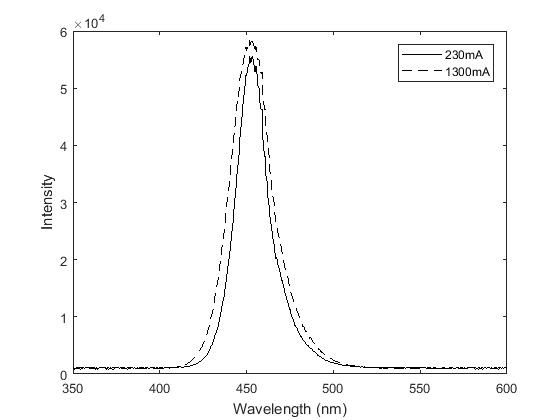
\includegraphics[width=0.6\linewidth]{figures/spektralanalys_mightex455nm}
\caption{Spectrum of the Mightex 455nm LED using two different driving currents. The band width is slightly wider for the higher current.}
\label{fig:ledspectrum}
\end{figure}

\subsection{Laser Light}

Using coherent light for imaging means that the effects of interference patterns will dominate the image of small particles. This is e.g. used when reconstructing images in holographic imaging instruments mentioned in section \ref{sec:relwork}. Laser illumination was tried used using two wavelengths, 450 and 850 nm. The images using laser illuminating the sample from an angle 

\subsection{Image Noise}

The total image noise was first measured using the whole image using the 455nm LED light, resulting in a variation coefficient of about nine percent.

The idea came that we should be able to measure the signal to noise relation, if the shadow image of the droplet is represents the signal. This signal to noise ratio (SNR) could possibly be used to increase the accuracy of the measurement. A function was created that calculates the noise level locally around each analyzed droplet image. A correlation could be seen between the SNR and the corresponding measuring range, resulting in an increased sampling volume for higher SNR. This relation has not been implemented in the LWC calculation for the prototype instrument yet.

The SNR for a ten micrometer dot image was compared for the different available gain level settings in the image sensor. This measurement was done using both the 455 and the 850 nm illumination. The result can be seen in Figure \ref{fig:noisegain}.

\begin{figure}%[ht]
\centering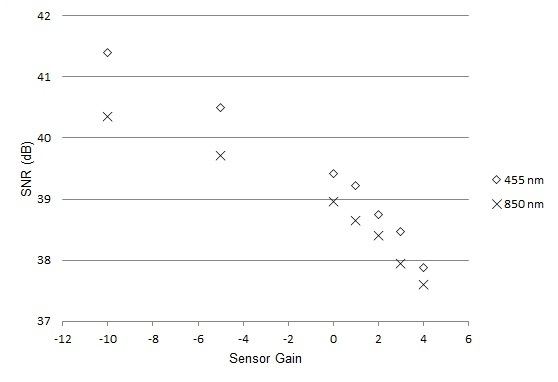
\includegraphics[width=0.6\linewidth]{figures/NoiseGain}
\caption{SNR for a ten micrometer dot image using two wavelengths and seven gain level settings. Shorter wavelength and lower gain gives less noise.}
\label{fig:noisegain}
\end{figure}

\subsection{Ambient Light}

In daylight, there is always some ambient light. Although the camera is never aimed direclty at the sun and the system make use of a telecentric lens we wanted to be sure that this light is not enough to affect the measurement. To get an idéa about the amount of ambient light the camera and lens was tested alone in daylight, using a fog generator in front of the lens to reflect light into the lens. 

The shortest possible exposure time according to the camera specification is 0.038 ms, slightly depending on other camera settings. For each measurement 152 images were captured, with increasing exposure time from 0.040635 to 1.988535 ms. A delay of 1 second was set between each image. Figure \ref{fig:ambientlight} shows the mean pixel value and the standard deviation of the value for one of the measurements at 22000 lux ambient light.

\begin{figure}%[ht]
\centering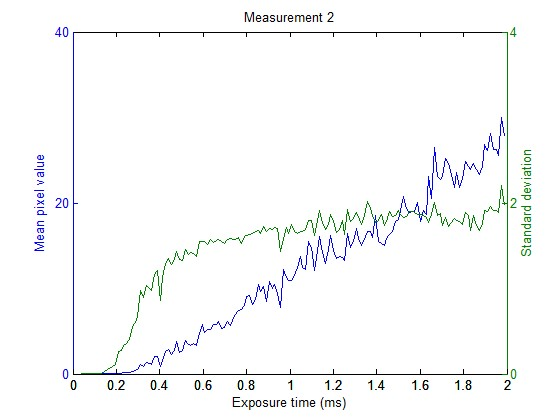
\includegraphics[width=0.6\linewidth]{figures/Amblight22000lux}
\caption{Mean pixel value and standard deviation of ambient for a light measurement at 22000 lux.}
\label{fig:ambientlight}
\end{figure}

Using this setup it was found that an exposure time of at least one second is needed to give a signal that is comparable to the noise level in a normal exposure. In order to image small droplets, the exposure time needs to be less than one μs, preferrably less. This difference is greater than the 8-bit pixel resolution used ($2^8=256$).

\subsection{Light Sensitivity Measurement}

The illumination energy required to get a good exposure for each of the eight gain setting levels is shown in Fig. 9. 34 nJ is required for the area in view (7.8 $mm^2$) for the lowest gain setting, which results in the highest SNR. The area in view is about 8 times smaller than the illuminated area of the collimated LED, which was measured to about 8x8 mm. 

\begin{figure}[ht]
\centering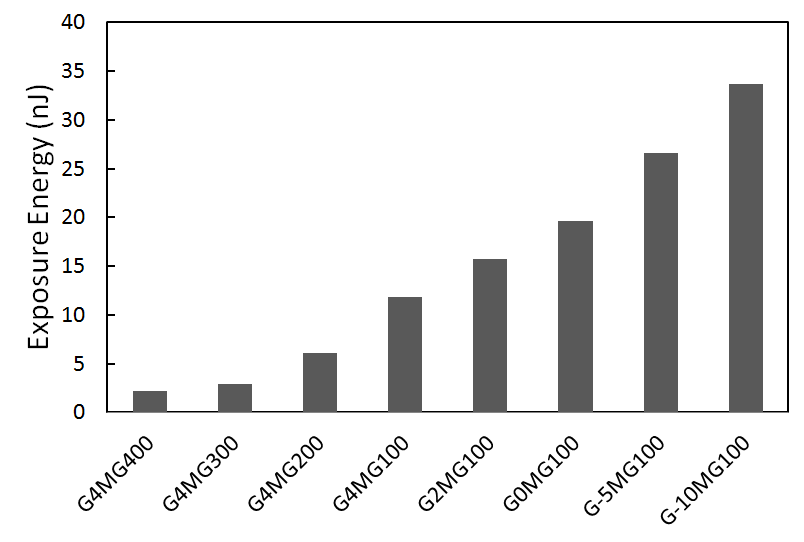
\includegraphics[width=0.75\linewidth]{figures/Energy_per_gain_level2}
\caption{Light energy ($nJ$) for exposure in each of the eight gain levels used. The energy was tuned manually up to a level of high exposure, but not saturating any point in the image.}
\end{figure}


\section{Design Considerations}

\subsection{Speed of Light Flash}

A value of both MVD and LWC can be derived from a series of images and since the number of measured droplets will depend on the concentration, the accuracy and precision will depend on the number of samples from the total population of droplets. 

The illuminative power required to get a good exposure is tested.

\section{Calibration and Validation of the Calibration}

The system is calibrated using a stage micrometer scale with 13 circular dots printed in chrome on a silicon glass. The dots range from 2 to 100 μm in diameter. Each dot is moved linearly in steps of one micrometer in the direction orthogonal to the lenses, thus creating a function where the gradient of the edge depends on the distance from optimum focus. A threshold on the second derivative gradient strength limits the measured particles to be within a specific measuring range. It is important to select the threshold carefully. If the value of the threshold is too low, there will be many false edges in the image. If it is too high, the measuring range will be too small. The difference between two different thresholds, 0.002 and 0.005 is illustrated by Figure \ref{fig:measrangevslogth}.  The measuring range is here defined as the distance in which the edge detection by Laplacian of Gaussian operator and a threshold makes a closed curve in the resulting binary image.

\begin{figure}[ht]
\centering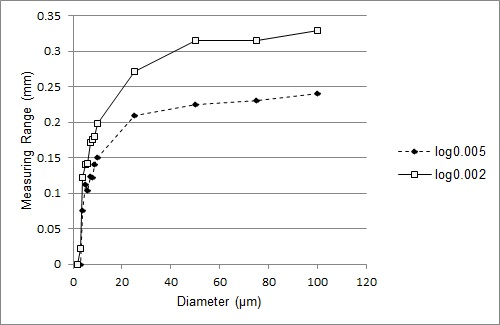
\includegraphics[width=0.75\linewidth]{figures/meas_range_vs_log_th}
\caption{Measuring range (mm) vs. diameter for two different thresholds (0.005 and 0.002).}
\label{fig:measrangevslogth}
\end{figure}

The edge sharpness will affect the position of the edge and the measured shadow slightly. We use the maximum value of the second derivative $P_{i,j}$ for each droplet as a measure of the edge sharpness and include this in the calibration functions, together with the diameter measured from the shadow intensity.

Two second degree approximation surfaces, (\ref{eq:z1}) and (\ref{eq:z2}), are calculated using the “fit” command in Matlab. $z_1$ approximates dot diameters from 2 to 10 micrometers and $z_2$ diameters from 10 to 100 micrometers. x is the maximum second derivative, $d^M$ is the diameter measured from the shadow intensity, $p_{xx}$ and $q_{xx}$ are constants.

\begin{equation} \label{eq:z1}
z_1=p_{00}+p_{10} x+p_{01} d^M+p_{20} x^2+p_{11} xd^M+p_{02} {(d^M)}^2
\end{equation}
\begin{equation} \label{eq:z2}
z_2=q_{00}+q_{10} x+q_{01} d^M+q_{20} x^2+q_{11} xd^M+q_{02} {(d^M)}^2
\end{equation}
By measuring the calibrated microspheres a validation can be made with the expected diameter. 

\subsection{Verification of Dot Size}

The dots on the micrometer scale were measured visually using a Leica microscope connected to a digital camera. This was done to get accurate values of the diameter of the dots for use in the calibration. An example image that was measured can be seen in \cref{fig:50umdot40x}.

\begin{figure}[ht]
\centering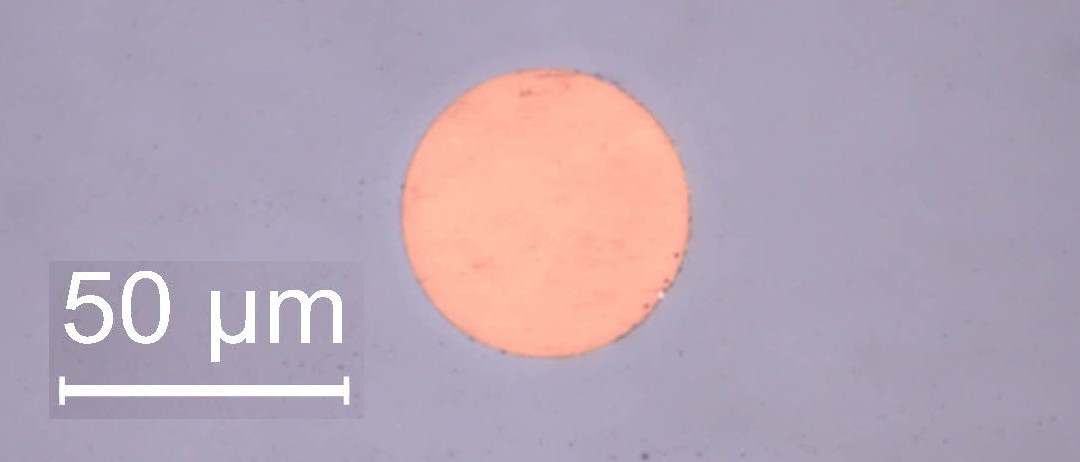
\includegraphics[width=0.75\linewidth]{./figures/50umdot40x.jpg}
\caption{The 50 micrometer dot with front illumination imaged using 40x magnifying lens.}
\label{fig:50umdot40x}
\end{figure}

This measurement was done using lenses with two different magnifications: 40x and 100x. All the dots average diameters, except the 100 µm dot were found to be within $\pm$ 0.2 $\mu$ m of their nominal diameter. They are not all perfectly round, but the size accuracy should be good enough to use as calibration reference. The result from this measurement is comprehended in \cref{tab:ref_meas}.

\begin{table}[ht]
\centering
\begin{tabular}{p{0.2\linewidth} p{0.2\linewidth} p{0.2\linewidth} p{0.2\linewidth}}
\hline
\textbf{Nominal Diameter} & \textbf{Excentricity} & \textbf{Diam. 40x} & \textbf{Diam. 100x} \\
\hline
5 & 0.2 & 5 & 4.8 \\
6 & 0.6 & 5.8 & 5.8 \\
7 & 0 & 7 & 6.6 \\
8 & 0 & 8 & 7.9 \\
9 & 0 & 9 & 8.8 \\
10 & 0 & 10.1 & 9.8 \\
25 & 0 & 24.9 & 24.7 \\
50 & 0.4 & 50.1 & 49.8 \\
75 & 0.2 & 75.2 & 74.8 \\
100 & 2.5 & 100 & 98.7 \\
\hline
\end{tabular}
\caption{Micro dot verification measurement. All values are in µm. Eccentricity is here the maximum difference in µm between the smallest and the largest measured diameter.}
\label{tab:ref_meas}
\end{table}


\section{The Shadowgraph System}

The instrument is a shadowgraph system using a monochrome CMOS camera with a 4x magnifying telecentric lens and a LED with a collimating lens illuminating the background. The blue LED is powered by a current driver able to produce short 12 A current pulses. Figure \cref{fig:shadowprinc} shows a sketch of the system. 

The system is mounted in a weather proof shell using two standard camera housings and a separate box for the analyzing computer and power supply. Fig. 2 shows the system mounted in weather proof camera housings. 

\begin{figure}[ht]
\centering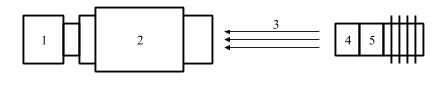
\includegraphics[width=0.75\linewidth]{./figures/shadowprinc.jpg}
\caption{Principle of shadowgraphy. 1. Camera. 2. Telecentric lens. 3. Parallell focused light beam. 4. Collimating lens. 5. LED.}
\label{fig:shadowprinc}
\end{figure}

\begin{figure}[ht]
\centering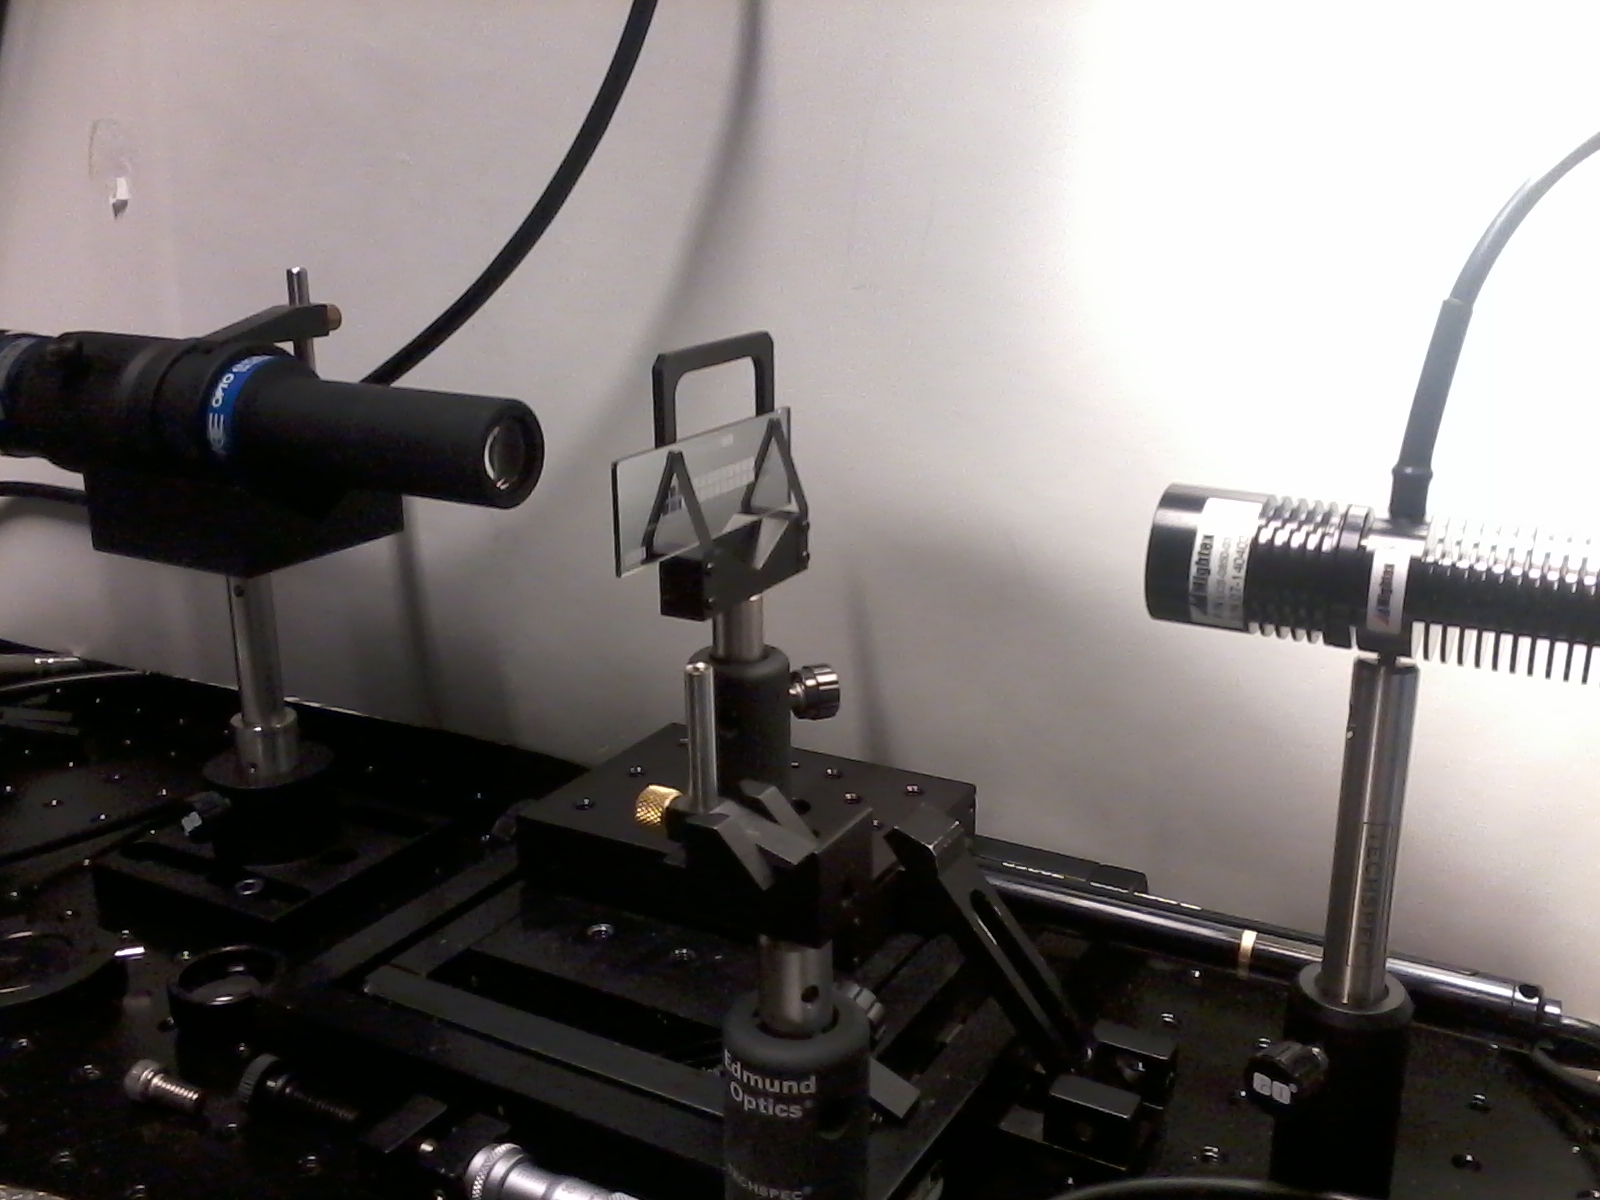
\includegraphics[width=0.75\linewidth]{figures/Foto0169}
\caption{The experimental setup with a dot micrometer scale as test object mounted on a translation stage.}
\end{figure}

\begin{figure}[ht]
\centering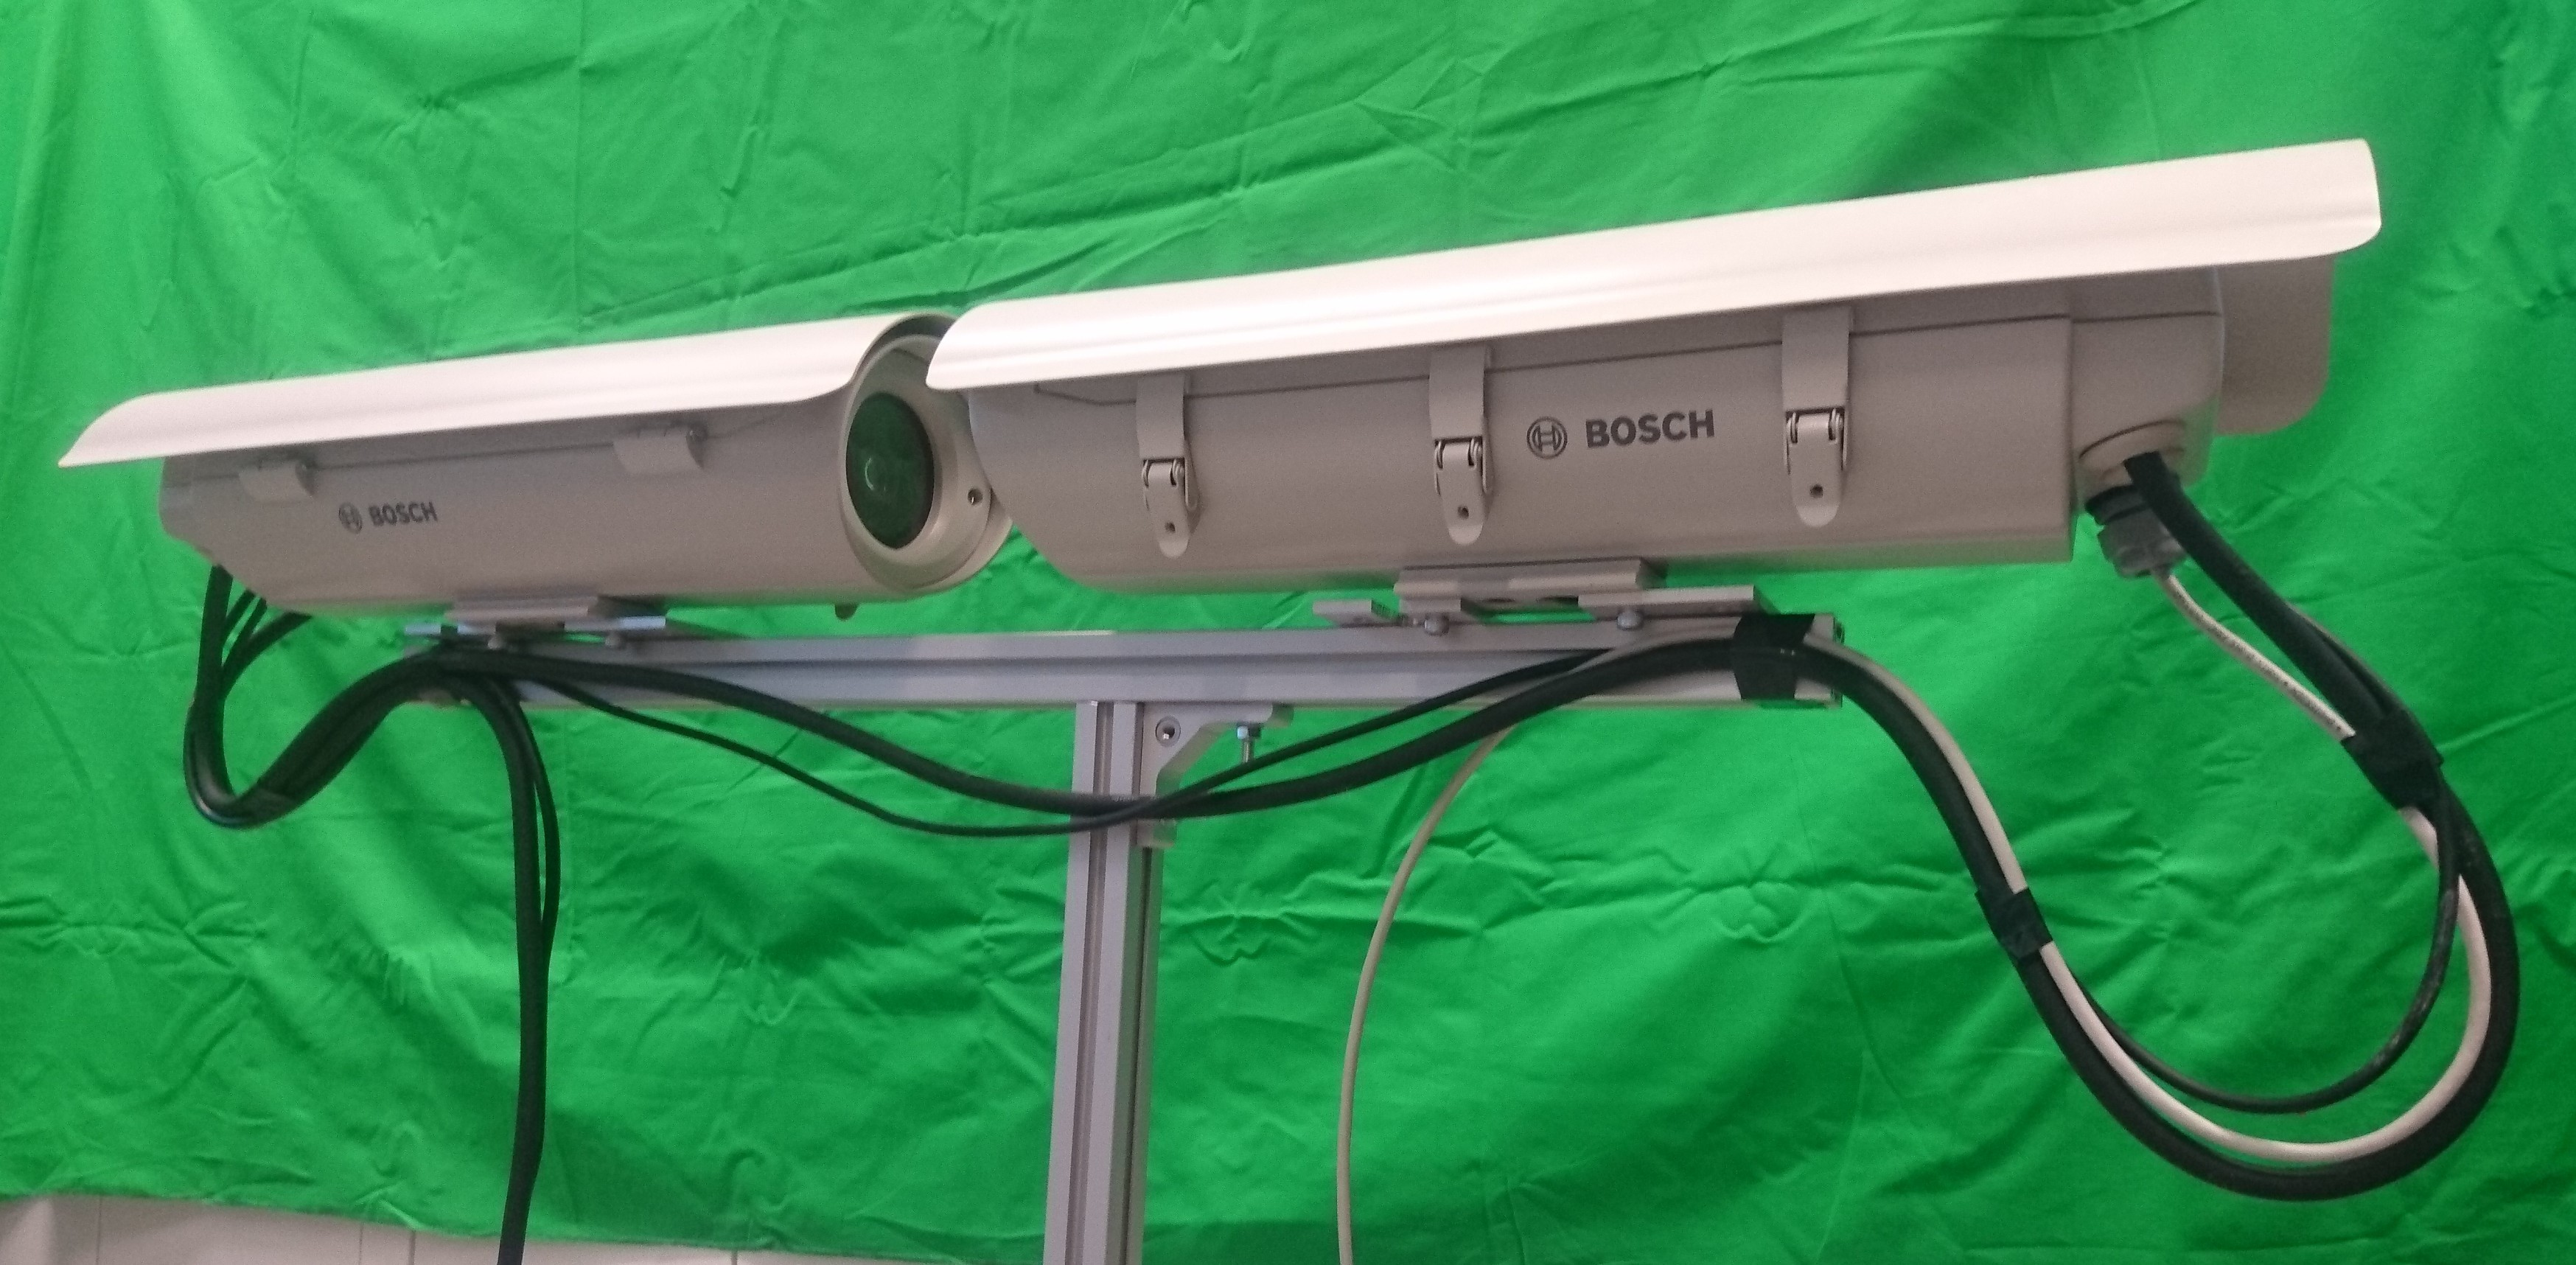
\includegraphics[width=0.75\linewidth]{figures/cam_housings}
\caption{The illumination and detector is mounted inside two Bosch camera housings facing each other with heating inside the house and on the front glass.}
\end{figure}

Calibration of true droplet size and measuring range both depends on the measured size of the droplet shadow and the amount of light used for exposure. It is possible to predict both the precision of the measured size and accuracy for measurement of droplet size. 

We used a stage micrometer scale for characterization of the system and simulation of water droplets. This characterization holds true given that the optical silhouette of a droplet is comparable to a dot having equal diameter and being printed on a silicon glass. It is not a new concept and has at least once been proved experimentally, by comparing with beads of glass and water droplets of known sizes \cite{koro1991,koro1998}. The shadow image of water drops of any size will be defined mainly by the diffracted component, as long as the distance between the drop and the lens is much larger than the drop diameter \cite{koro1991,wend2013}. 

The design using a weakly collimated LED that illuminates an area slightly larger than the field of view makes the system quite insensitive to misalignment of the camera and the light source. Temporal or permanent changes in light intensity caused by a minor misalignment is automatically compensated for by continuous measurement of the total exposure level. If the level of exposure is increasing or decreasing, the length of the light pulse is changed correspondingly. The light intensity can also be affected by dirt on the front glass of the housings. 

Since many images will not contain any droplet at all, we can increase the processing speed by sorting out the images that are not containing any interesting information. This is done by constructing an average image from 20 images and use this as a flat-field correction. All new images are compared with this average and if any pixel differs from the average by more than a specific value that is significantly higher than the noise level, the image is analyzed.

Spatial dissimilarities in the light intensity that are not caused by noise are compensated for by calculating the local average intensity of the background around each measured droplet. The size of a droplet is then based on the intensity dip caused by the shadow compared with its local background.

\subsection{Exposure Check and Flash Intensity Adjustment}

Let $I_{i,j}$ depict the two dimensional image captured by the camera. The mean value $\overline{i}$ of all pixels in the image $I_{i,j}$ gives an estimation of the exposure level in the whole image. 

The flash duration is adjusted automatically by the microcontroller at each exposure to keep the exposure level between a low and a high threshold, $th_L$ and $th_H$. The duration is changed in steps of 13 ns corresponding to one clock cycle of the microcontroller. If $\overline{i} > th_L$ and $\overline{i} < th_H$ the image is analyzed. If $\overline{i} \geq th_H$ the flash duration is decreased by steps of 12 ns. If $\overline{i} \leq th_L$ the flash duration is increased. The total flash duration is approximately 250 ns. $th_L$ is here set to 0.7 and $th_H$ is set to 0.8 in a normalized (0,1) dynamic range.

\subsection{Edge Detection and Edge Sharpness}

To detect the intensity changes created by the shadow of a water droplet, an image is processed using the from edge detection theory well known Laplacian of Gaussian (LoG) described by Marr and Hildreth \cite{marr1980}. The method works by looking for zero crossings in the image resulting from calculating $\nabla^2 G\left(x,y\right) * I\left(x,y\right)$. $G\left(x,y\right)$ is a two dimensional Gaussian distribution with standard deviation σ and $\nabla^2$ is the Laplacian operator, defined as the divergence of the gradient in two dimensions.
\begin{equation}
G\left(x,y\right) = \frac{1}{\pi \sigma^2} e^{-\frac{x^2+y^2}{2\sigma^2}}
\end{equation}
\begin{equation}
\nabla^2=\nabla\cdot\nabla=\frac{\delta^2}{\delta x^2} + \frac{\delta^2}{\delta y^2}
\end{equation}
We implement a discrete approximation to $\nabla^2 G\left(x,y\right) \approx \nabla^2 G_{i,j}$ as a 13x13 sized convolution kernel.
\begin{equation}
\nabla^2 G_{i,j} = -\frac{1}{\pi \sigma^4} \left(1 - \frac{i^2+j^2}{2\sigma^2} \right) e^{-\frac{i^2+j^2}{2\sigma^2}}
\end{equation}
By applying the convolution to the normalized image $I_{i,j}$ we get the resulting image $P_{i,j}$.
\begin{equation}
P_{i,j}=\nabla^2 G_{i,j} * I_{i,j}
\end{equation}
$P_{i,j}$ is thus a matrix that contains the second order derivative of the image $I_{i,j}$. 
A spherical object will cause an edge where the intensity change is similar around a spherical object, but dependent on the distance from the optimal focus. Assuming the Gaussian of the image I is twice differentiable at any point $(i,j)$, the maximum (or minimum) of the second derivative includes the amplitude of the first derivative at the point where the second derivative is equal to zero, i.e. where the edge is strongest. This can be intuitively understood when considering that if the edge is sharper, the gradient, or first derivative value is larger, and if the gradient value is larger the rate of change, i.e. the second derivative needs to be larger at each side of the edge. Therefore we store a value of the maximum second derivate, $max(P_{i,j}$, around each analyzed object and use this as a measure of the edge sharpness. This value is then used as input to a calibration function. 
We also construct a new binary image $Q$ in which the pixel value $Q_{i,j}=1$ if any of $|P_{i+1,j}-P_{i,j} |,|P_{i-1,j}-P_{i,j} |,|P_{i,j+1}-P_{i,j} |,|P_{i,j-1}-P_{i,j} |>th$, where $th=0.002$. $Q_{i,j}=0$ elsewhere. th is the gradient of the second derivative at the point where the second derivative is zero, i.e. on the edge. Particles are found by searching for closed contours in this binary image.

\subsection{Comparing Transparent Microspheres and Dots}

A spherical lens scatters almost all the incident light in different directions, leaving only a bright spot in the middle where light is transferred directly through. For larger particles in focus, this bright spot will result in a second circular closed contour inside the outer edge. 

Small water droplets can be seen as transparent microspheres. The composition changes the refractive index, but this has little effect on the shadow. The outer contour is the same following the same reasoning as with the dots used for calibration \cite{ryd2015}. Diffraction patterns depend on the wavelength of the light and the size of the sphere. The resolution of the constructed system is not high enough for these patterns to be visible.

By using a flood-fill function on the binary image containing the detected contour, starting in a point at a minimum distance from an object, the edge of the filled area will border to the outer contour. This makes it possible to select the outer closed contours of possible particles.

\subsection{Removing the Center Bright Spot}

The center bright spot will make the shadow of a transparent sphere brighter in average than a solid dot. This will have an impact on the size calculation, since the size calculation is based on the shadow impact and the calibration is done using solid dots. Therefore we apply a mask on the image before calculating the size of the shadow. The mask is done by replacing all the centermost pixels in a shape of a circular disc with the intensity of the darkest pixel in the spot. The diameter of the masked disc is the arc length of the edge contour divided by 4$\pi$. The bright spot is measured by calculating the difference between the least value and the center pixel. Only particles with a difference larger than 0.1 (ten percent) will have the mask applied

\subsection{Measuring Roundness}

There may be clogs of small microspheres or dust in the samples that are measured. Microspheres, or small water droplets are close to spherical. Therefore we try to exclude all objects that the program find but are not circular. After the detection of object edges, we measure the roundness of each object. A measure of the mean square roundness deviation similar to the one described by ISO \cite{iso12181} can be achieved by calculating the quote between the area of the contour and the square of the total arc length See (\cref{eq:5}).
\begin{equation}
roundness = 4\pi \frac{A_{contour}}{arcLength^2}
\label{eq:5}
\end{equation}
$A_{contour}$ is the pixel area of the contour and $arcLength$ is the perimeter of the measured closed contour. In the calibration and field measurements described, an object is only considered spherical if $roundness \geq 0.85$.


\section{The Fog Chamber}
The fog chamber is needed to create a test environment for the instrument. Natural fogs tend not to occur outside just when we are ready to test. If possible, it is desirable that the environmet can be controlled and verified using a second instrument. It gives an indication of how the instrument will behave in a real measurement. It is also a verification of the instrument’s water ingress resistance.

The constructed chamber has a frame made of 30 mm aluminum profiles, fitted with transparent 6 mm polycarbonate walls on all sides using rubber sealing strips. The droplets are produced using an ultrasonic fog generator pushing the droplets to the chamber through a flexible tube approximately 30 mm in diameter and 500 mm long. Next to the fog inlet, there is a dry air inlet with a speed adjustable fan. On the back of the chamber there is a similar sized outlet for air and moisture.
 
\begin{figure}[ht]
\centering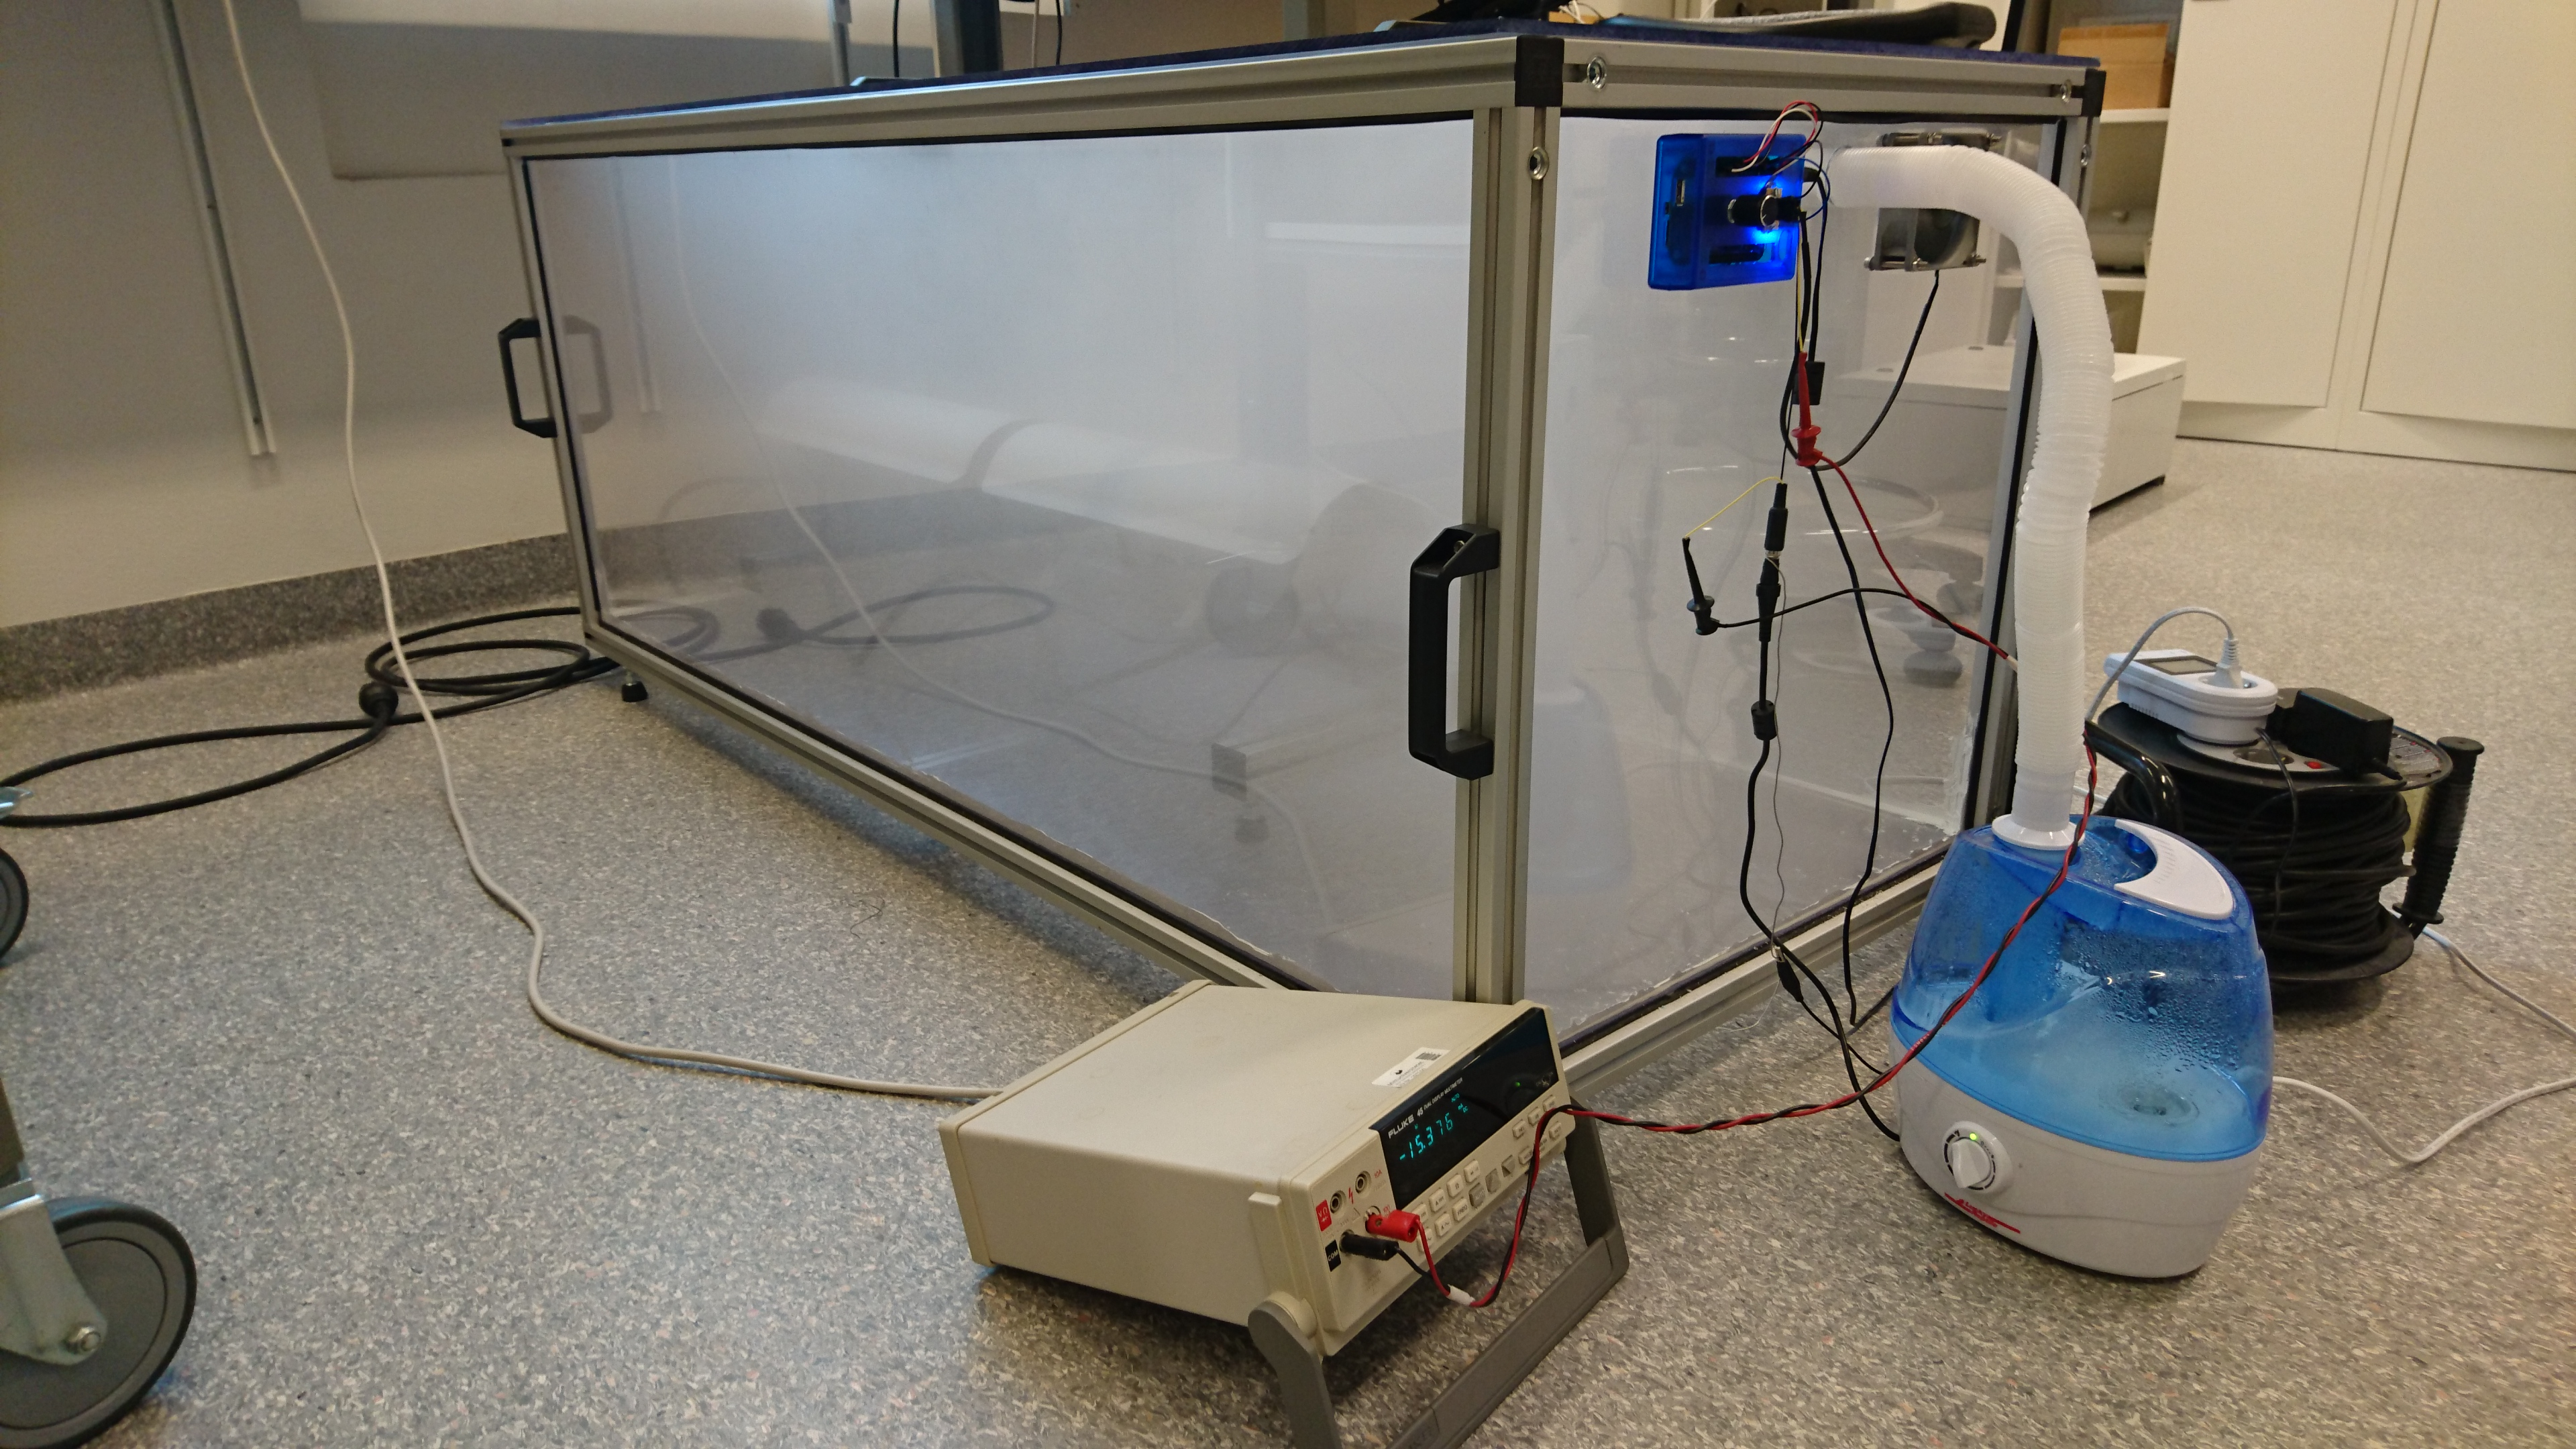
\includegraphics[width=0.75\linewidth]{figures/DSC_0103}
\caption{Fog chamber with connected droplet generator (blue container) and a multimeter used for fan power measurement. A Beaglebone Black microcontroller (blue box) is used for fan speed regulation.}
\end{figure}

\section{The Klövsjö Installation}
Figure \ref{fig:installation1} shows the installation. On top is the two camera houses of the DII and just below is the smaller CDP. The Lambrecht Eolos weather sensor is seen furthest to the left, mounted on an horizontal boom. In the middle just right of the Eolos is the mobile communication antenna. In the lower center the top of the shortened lattice mast is seen and behind this is the box containing the DII processing computer, the CDP data collection computer and the communications router. The whole installation is about five meters high. An electric servomotor mounted at the base of the pole inside the lattice mast rotates the two instruments automatically to follow the horizontal direction of the wind. 

\Cref{fig:installation3} shows icing on the front side of the installation.

\begin{figure}[ht]
\centering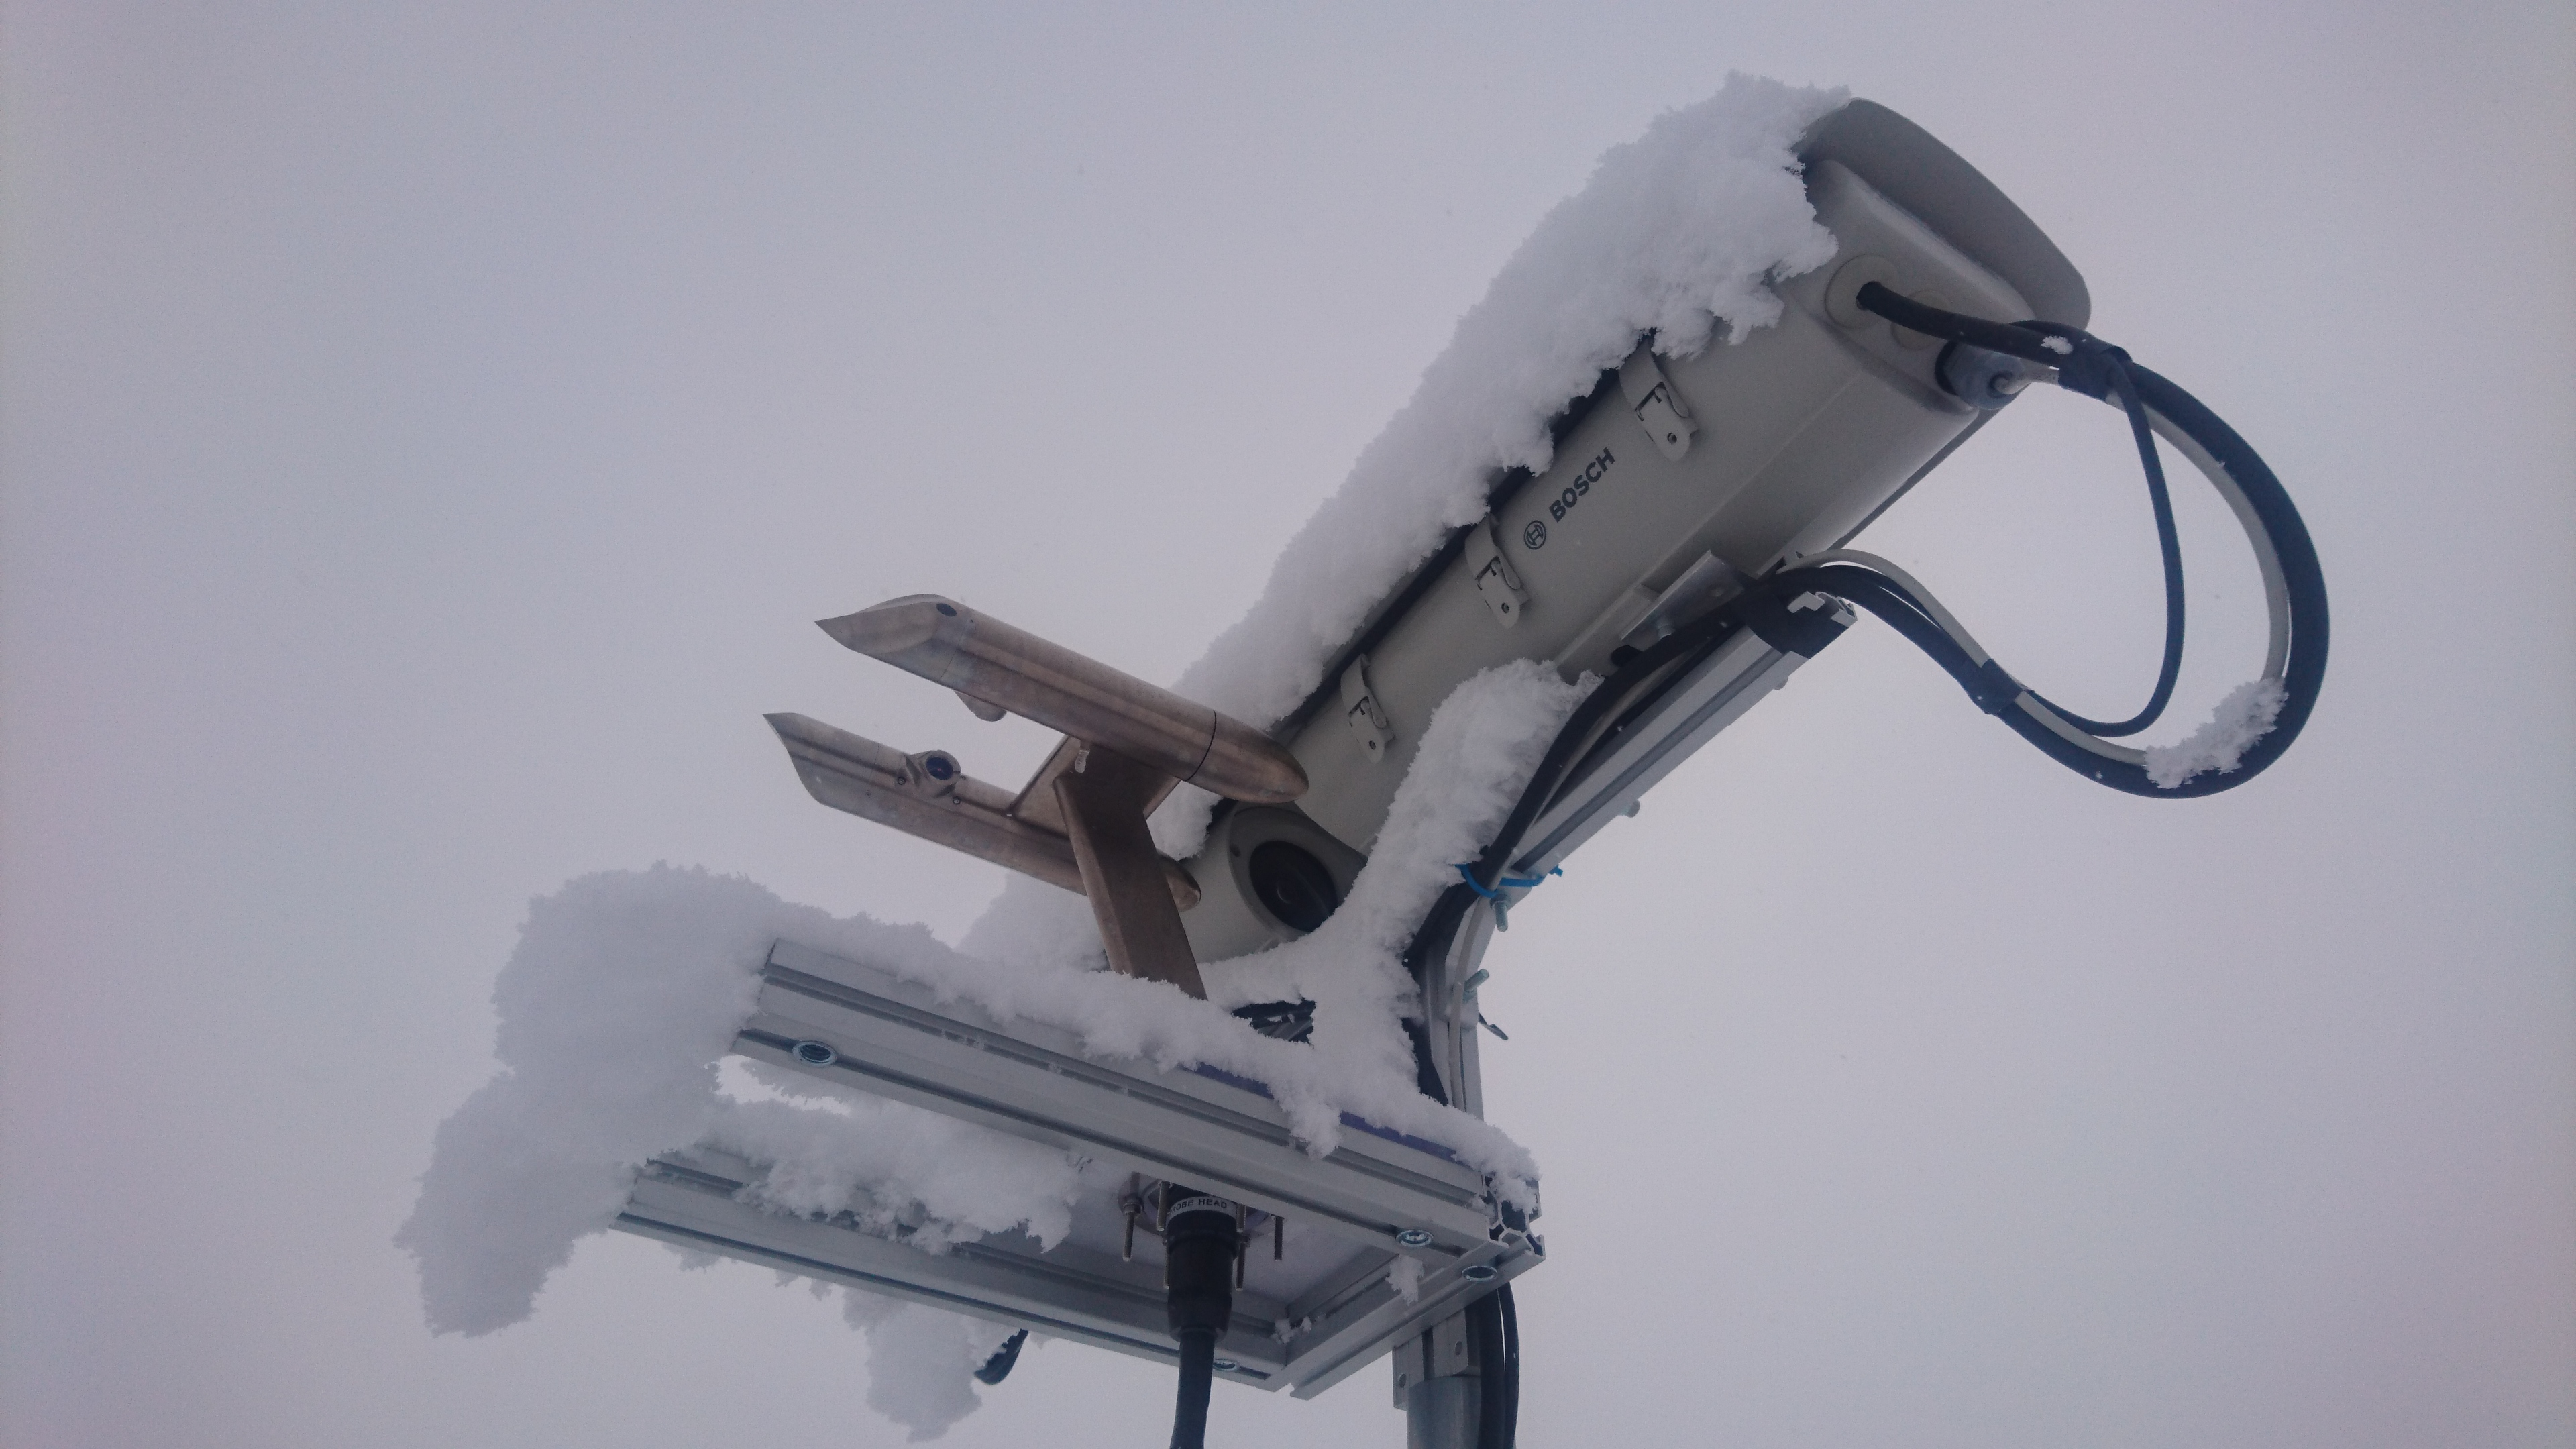
\includegraphics[width=0.75\linewidth]{figures/installation3}
\caption{Icing on the front side of the installed instruments.}
\label{fig:installation3}
\end{figure}

\begin{figure}[ht]
\centering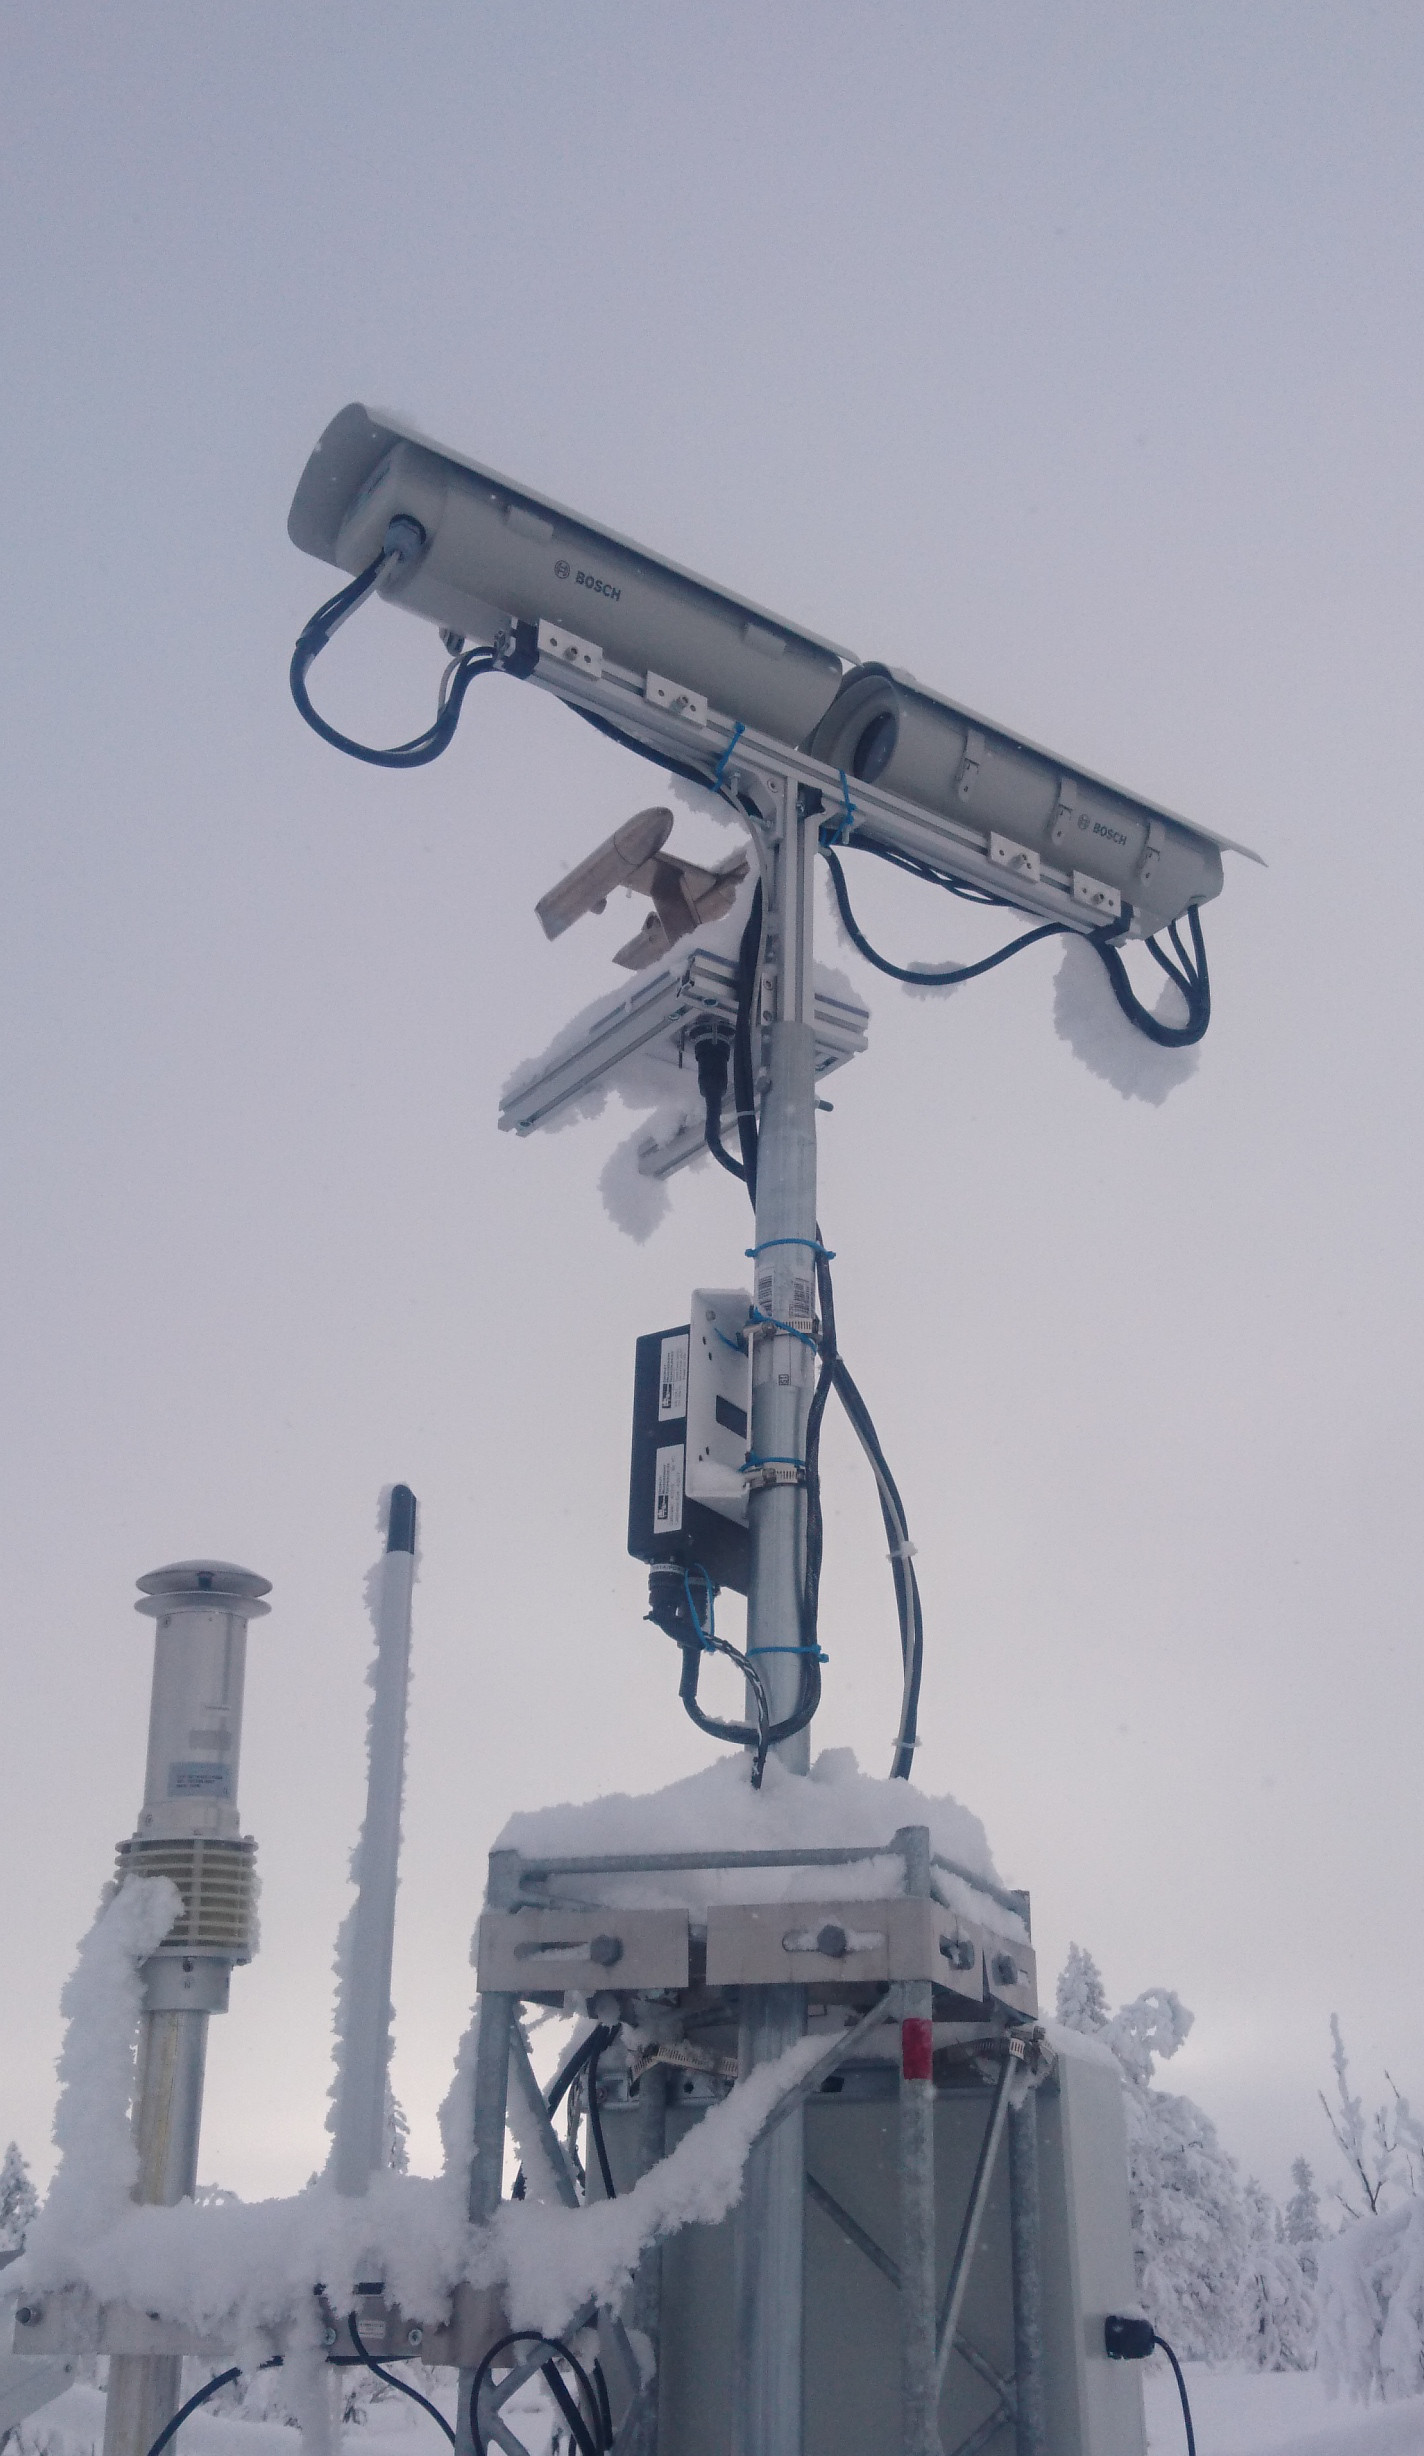
\includegraphics[width=0.75\linewidth]{figures/installation1}
\caption{Installation in Klövsjö.}
\label{fig:installation1}
\end{figure}

% this is shows the paper size and measures
%\begin{figure}
%    \oddpagelayouttrue
%    \twocolumnlayoutfalse
%    \stockdiagram
%    \caption{Right-hand page major layout parameters for
%        the \file{memoir} class} \label{fig:mempplt}
%\end{figure}
%\stockvalues